%!TEX root = ../main.tex

\chapter{Background}
\label{sec:background}

\section{Separation Logic - theory and tooling}
\label{sec:background:sl-and-tools}

Proposed in 1969, Tony Hoare's \textit{Hoare Logic} provided a standardised
means of reasoning about programs and their correctness~\cite{hoare}. The key
principle of this logic is the Hoare Triple, denoting that if a certain
pre-condition $P$ holds, and code command $C$ is run (and terminates without
failing), then the post-condition $Q$ is guaranteed to hold. This is presented
in the form of a \textit{H ffoare triple}:
$$
  \triple{P}{C}{Q}
$$

Whilst this is a strong foundation for reasoning about programs, anything more
than the simplest of functions become hugely cumbersome to work with,
particularly concerning operations on heap-allocated memory. In 2001, Peter
O'Hearn and John Reynolds proposed \textit{Separation Logic} as the solution to
this~\cite{separation-logic}. Separation Logic reasons about
\textit{heap fragments} (sometimes called \textit{heaplets}), which represent
sections of a theoretical computer's heap; it also provides three core features
in addition to the standard Hoare Logic:

\begin{figure}[!b]
  \centering
  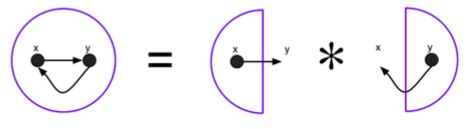
\includegraphics[width=200px]{img/separating-conjunction.jpg}
  \caption{
    A visualisation of the separating conjunction.
    From~\cite{infer-sl}.
  }
  \label{fig:separating-conjunction}
\end{figure}

\begin{itemize}
  \item The \textit{heap cell assertion}, $\cell{x}{y}$, denotes that a heap
  fragment composes of a single cell at address $x$ with value $y$.

  \item The \textit{separating conjunction}, $P \lstar Q$, states that the heap
  fragment can be split into two disjoint (potentially empty) sub-fragments,
  one of which satisfies $P$, and the other satisfies~$Q$.

  \item The \textit{Frame Rule} - a fundamental rule that allows derivations to
  temporarily ``forget'' any unneeded logic either not concerning
  heap-allocated memory, or concerning heap-allocated memory that isn't mutated
  by the command(s) currently being considered. Intuitively, this states that
  any programs that can execute on a state $P$ can also execute on a larger
  state, $P \lstar R$. The Frame Rule is as follows:

  $$
    \inferrule[Frame]{
      \triple{P}{C}{Q} \quad \mathtt{mod}(C) \cap \mathtt{fv}(R) =
      \emptyset}{\triple{P \lstar R}{C}{Q \lstar R}
    }
  $$
\end{itemize}


Separation logic made its first foray into automatic analysis tools with the
creation of \textbf{Smallfoot}~\cite{smallfoot-paper, smallfoot-site}. It works
on a small while language with static objects, requiring pre- and
post-conditions and loop invariants, and has the ability to reason about simple
data structures such as lists and trees.

The utility of separation in tooling was expanded with the development of
bi-abudction techniques; bi-abduction is a method of symbolic program analysis
that can automatically infer the pre- and post-condition of functions.
\textbf{SpaceInvader} was introduced with the ability to infer some loop
invariants in small C code, with \textbf{Abductor} later added to introduce
bi-abduction to the toolset~\cite{abductor}.

2011 saw the intrudoction of \textbf{VeriFast}~\cite{verifast-paper,
  verifast-repo}, `a prototype verification tool for single-threaded and
multi-threaded C and Java programs'. VeriFast performs verification similar to
Gillian, working on functions with developer-defined pre- and post-conditions,
also using an intermediate representation to do so. Figures
\autoref{fig:verifast-example} and \autoref{fig:verifast-example-output} show how
VeriFast handles a small Java program that deliberately dereferences a null
pointer.

\begin{figure}
    \centering
    \begin{lstlisting}[language=Java,
        style=code,
        xleftmargin=0.2\textwidth,
        xrightmargin=0.2\textwidth]
class VerifastTest \{
    int nullDeref()
        //@ requires true;
        //@ ensures 0 <= result;
    \{
        String str = null;
        return str.length();
    \}
\}
    \end{lstlisting}
    \caption{\texttt{VerifastTest.java}}
    \label{fig:verifast-example}
\end{figure}

\begin{figure}
    \centering
    \begin{lstlisting}[style=terminal,
        xleftmargin=0.05\textwidth,
        xrightmargin=0.05\textwidth]
> verifast ./VerifastTest.java
./VerifastTest.java
./VerifastTest.java(7,20-26): Target of method call might be null.
    \end{lstlisting}
    \caption{Output from analysing \texttt{VerifastTest.java}}
    \label{fig:verifast-example-output}
\end{figure}

In industry, probably the most prominent use of a tool built on separation logic is Facebook's \textbf{Infer}~\cite{infer, infer-site}; it's a static analysis
tool for Java and C/C++/Objective-C, designed to use bi-abduction to provide
users with a list of potential bugs, crashes, and sources of poor performance.
Similarly to Gillian, Infer is written in OCaml, and works by compiling source
code to an intermediate representation. In contrast, Infer wholly focuses on
automated compositional testing, and refines this process to a state in which
it can easily be used in industry, whilst also including more general analysis
for concerns such as security and concurrency; it sacrifices depth of analysis
to result in a lightweight tool that gives developer-friendly feedback.
Infer doesn't require the a full program in order to perform analysis, as it
only needs to construct Hoare triples for one function at a time. This,
combined with its ability to reuse existing results from unchanged functions and
only consider modified code, makes for a fast and hugely scalable static
analysis tool, used as part of Facebook's code quality pipeline for all
modifications to the Android and iOS apps for Facebook, Facebook Messenger,
Instagram, and others services~\cite{infer-about}. Infer outputs discovered
errors and warnings to a file in CSV, whilst directly outputting the most
severe. \autoref{fig:infer-example} and \autoref{fig:infer-example-output} show
a short example of running Infer on a similar function to what was tested with
VeriFist.

\begin{figure}
    \centering
    \begin{lstlisting}[language=Java,
        style=code,
        xleftmargin=0.2\textwidth,
        xrightmargin=0.2\textwidth]
class InferTest \{
    // Deliberately call a method on a null pointer
    int nullDeref() \{
        String str = null;
        return str.length();
    \}
\}
    \end{lstlisting}
    \caption{\texttt{InferTest.java}}
    \label{fig:infer-example}
\end{figure}

\begin{figure}
    \centering
    \begin{lstlisting}[style=terminal,
        xleftmargin=0.05\textwidth,
        xrightmargin=0.05\textwidth]
> infer -- javac ./InferTest.java
Starting analysis (Infer v0.5.0)

... (skipping some lines) ...

Found 1 issue
InferTest.java:5: error: NULL_DEREFERENCE
  object str last assigned on line 4 could be null and is
  dereferenced at line 5.
  3.       int nullDeref() \{
  4.           String str = null;
  5. >         return str.length();
  6.       \}
  7.   \}
    \end{lstlisting}
    \caption{Output from analysing \texttt{InferTest.java}}
    \label{fig:infer-example-output}
\end{figure}

Both VeriFast and Infer produce clear and direct feedback about the null
dereference error, providing line numbers (and even column numbers, in
VeriFast's case) and a clear cause of the error.

\subsection{Reaching beyond separation logic}

Currently, Infer is not limited to using separation logic -based techniques for
bug finding, developing checks that make use of various other program analysis
in order to broaden the scope of errors that Infer can report, through the use
of \textbf{abstract interpretations}; this entails the exploration of all
possible states of a program through a series of over-approximations (a deeper
understanding is outside the scope of this project).

A strong source of inspiration for Infer's abstract interpretation techniques is
\textbf{Frama-C}~\cite{frama-c-paper, frama-c-site}, `a source code analysis
platform that aims at conducting verification of industrial-size C programs'; a
noteworthy feature of Frama-C is its debugger-esque graphical interfaces
available for certain analyses.


\subsection{Debugging}

Whilst the depth of analyses via separation logic has increased over the years,
clarity of error reporting remains difficult to maintain. Until recent work on
Gillian by Matthew Ho~\cite{gillian-debugging-2021}, VeriFast's clear-cut
advantage over similar tools was its functioning debugger, and succinct,
immediate error reporting; as found in previous
comparisons~\cite{gillian-logging-2020}, upon attempting to verify an invalid
program, VeriFast will directly output its reasoning for the error, and the line
number responsible. VeriFast remains ahead of Gillian's debugging capabilities -
whilst the work of Ho from 2021 markedly closed the gap between the two tools
(and provided more specific and helpful error reporting, in Gillian, as well as
some ease-of-use features such as debugging specific functions), the DAP's
limitations on Gillian debugging left for some sorely missed features, such as
the VeriFast debugger's ability to jump to any symbolic execution step, and
visually show when resources allocated on the heap are freed. As of the
beginning of this project, the ability to select execution branch when debugging
is absent from both Gillian and VeriFast.
\autoref{fig:verifast-debugging-example} shows VeriFast's debugging interface.

\begin{figure}
  \centering
  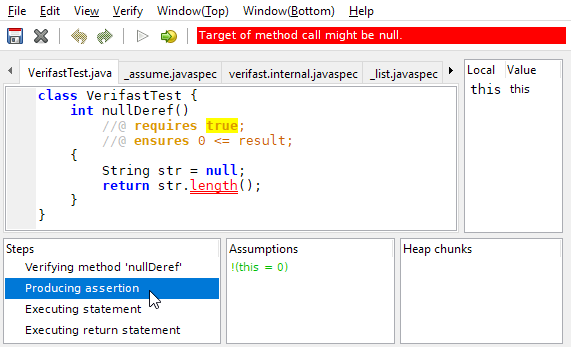
\includegraphics[width=0.75\textwidth]{img/verifast-debugging-example.png}
  \caption{
    An example of VeriFast's debugging interface, using the program from
    \autoref{fig:verifast-example}
  }
  \label{fig:verifast-debugging-example}
\end{figure}


\section{Gillian}

\section{Engieneering resources and tools}
\label{sec:background:engineering-tools}

Due to the nature of the project, some research into the language and tools that
are (or could/will be) used in Gillian was worthwhile.

\subsection{Building OCaml projects}

Created in 1996, \textit{OCaml}~\cite{ocaml} is `an industrial-strength
programming language supporting functional, imperative and object-oriented
styles'. Specifically, OCaml provides the ability to make use of functional,
imperative, and object-oriented styles. This, combined with its powerful type
system, makes it a good fit for symbolic analysis tools. Many of Gillian's
contemporaries, including Infer, VeriFast and Frama-C, are also written in OCaml.

OCaml's most popular build system is \textit{Dune}~\cite{dune} - it allows the
easy compilation of multi-file OCaml programs and libraries, including
dependencies from \textit{OPAM}~\cite{opam}, OCaml's designated public library
repository. Despite Dune's popularity, it is a fairly bare-bones system, quickly
growing cumbersome when developing larger projects and, in particular,
switching development between projects; Dune requires that OPAM dependencies
are installed system-wide, which can lead to inconsistent builds and version
conflicts. The answer to these concerns is \textit{esy}~\cite{esy}, a package
management system for OCaml and Reason styled after \textit{npm}~\cite{npm}.
Esy provides `provides a fast and powerful workflow for local development of
opam packages without requiring ``switches''', meaning dependencies are isolated
between projects. Esy also provides a number of convenience features, such as
defining custom commands that run within the OCaml project's environment, as
well as supporting non-OPAM dependencies, e.g. OCaml sources from GitHub
repositories (optionally at a specific commit).

Knowledge of these build systems will become paramount when introducing the
somewhat foreign element that is a VSCode extension.


\subsection{VSCode and its extensions}
\label{sec:vscode}

VSCode (Visual Studio Code)~\cite{vscode} is a universally recognised text
editor and development environment, developed by Microsoft. It currently stands
as the most popular development worldwide, enjoying a 71\% market share
according to Stack Overflow's 2021 developer survey
~\cite{stack-overflow-survey-editors}.

A large factor to VSCode's success is its extensive support for extensions,
boasting over 24,000 freely-distributed extensions~\cite{vscode-popularity},
ranging from language-specific support to general developer creature comforts
(such as SSH support). Developing new extensions is made very accessible through
simple JavaScript or TypeScript projects~\cite{vscode-extensions-intro}, making
use of VSCode's well-documented API~\cite{vscode-api} to have a large degree of
control over the editor.

Whilst VSCode limits the extent to which extensions can extend the editor's UI,
extension authors are able to make use of Webviews~\cite{vscode-webview}; an
extension can open an editor tab that contains web content (HTML/CSS/JS) that
the extension has complete control over, providing a method for extensions to
fill in any gaps in VSCode's UI.

\begin{figure}
  \center
  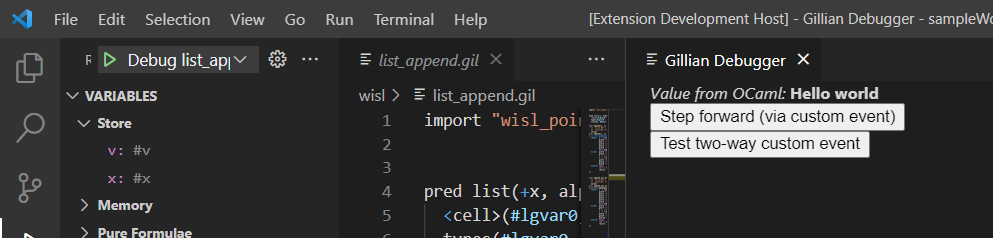
\includegraphics[width=400px]{img/webview-example.png}
  \caption{An example of a Webview created by a VSCode extension}
  \label{fig:webview-example}
\end{figure}


\myparagraph{Debug Adapter Protocol}
A common issue when adding IDE support for development tools is the sheer
number of editors that would ideally be supported~\cite{magpiebridge}. Whilst
VSCode has a huge market share, only supporting VSCode would neglect a
significant portion of developers. Unfortunately, maintaining support for many
editors at once is an unreasonably large undertaking. The \textit{Debug Adapter
Protocol} (DAP)~\cite{dap} exists as an attempted countermeasure to this issue,
turning the $O(m \times n)$ complexity problem of supporting many debuggers on
many editors into a $O(m + n)$ problem; each debugger and each editor need only
be integrated once.

\begin{figure}[!t]
  \centering
  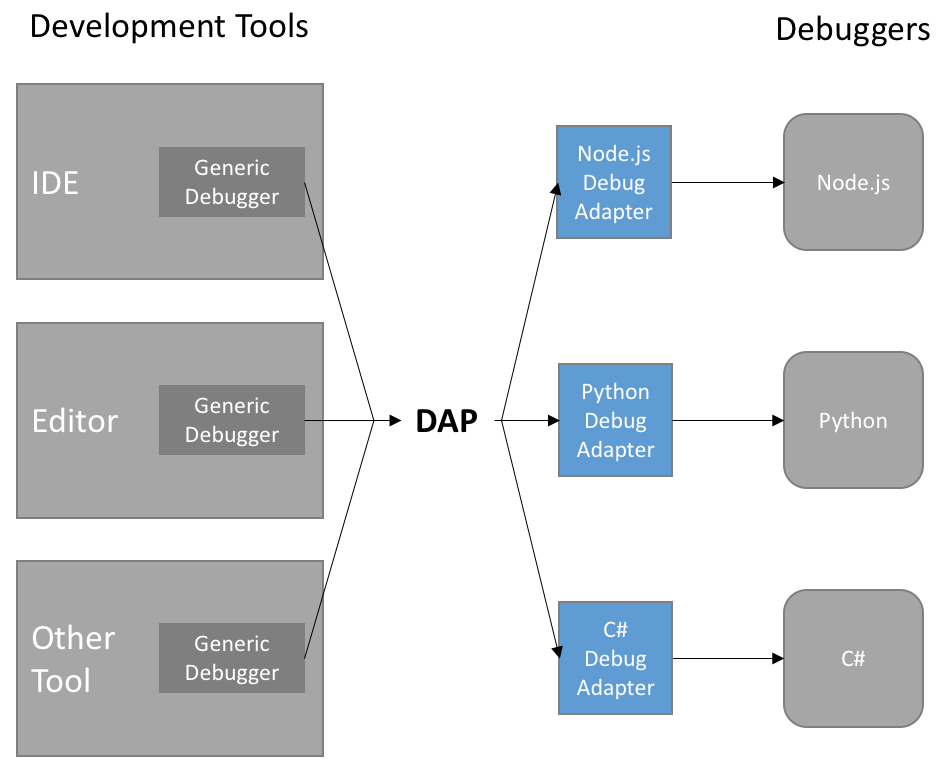
\includegraphics[width=0.5\textwidth]{img/dap-diagram.png}
  \caption{
    DAP: an interface between arbitrary IDEs and
    arbitrary debuggers~\cite{dap}.
  }
  \label{fig:dap-diagram}
\end{figure}

As discussed in \autoref{sec:intro}, the DAP's limited set of
included commands proved a limiting factor in the development of a Gillian
debugger. A potential solution is to make use of custom commands and events,
which is supported both by VSCode (sending custom requests
at~\cite{vscode-dap-custom-request}, receiving custom events
at~\cite{vscode-dap-custom-event} and the OCaml DAP
implementation currently used in Gillan's debugger~\cite{ocaml-dap} (where
custom events and commands are defined similarly to those already
provided~\cite{ocaml-dap-custom}).


\myparagraph{Inclusion of OCaml code}
Resulting of Ocsigen's work as part of their OCaml web framework
~\cite{ocsigen-framework}, OCaml programs can be directly compiled into
JavaScript using their \texttt{Js\_of\_ocaml} package~\cite{js-of-ocaml}; by
adding a compilation flag in a project's Dune file, the relevant program can be
compiled to a \texttt{.js} file instead of a native binary. This produced file
doesn't need to be used as its own program; using the provided JS
bindings~\cite{js-of-ocaml-bindings}, the resulting JS code can export
functions and values, just like normal JS code, to be used elsewhere in a
JavaScript project.

Another option is to make use of the OCaml VSCode bindings
~\cite{vscode-ocaml-bindings} provided by OCamlLabs'
\texttt{vscode-ocaml-platform}~\cite{vscode-ocaml-platform, ocamllabs}; this
way, no JavaScript need be written at all.

These options allow the line between JavaScript and OCaml to be drawn wherever
is most opportune; the extension could be written completely in JavaScript,
requiring more attention when interacting with Gillian's debugger; the
extension could be entirely OCaml, sacrificing more succinct integration with
VSCode for a more unified codebase with Gillian; it is just as possible to draw
the line somewhere in-between, exposing the more Gillian-related OCaml code via
functions to the JavaScript that communicates with VSCode. Additionally, both
scenarios allow for Gillian code to be shared with the extension. However,
with the Gillian libraries as they are, such libraries cannot be haphazardly
included in the extension code; \texttt{Js\_of\_ocaml} transitively includes all
OCaml dependencies, potentially leading to code that cannot be executed. As a
concrete example to this, attempting to include Gillian's \texttt{debugAdapter}
library results in erroring code, due to the compiler's attempt to include an
SQLite implementation, which it simply is not equipped to handle. Aside from
this, the inclusion of unnecessary dependencies in JS-compiled code results in
a hugely bloated extension - the \texttt{debugAdapter} example created a
compiled JS file over a million lines long. The ideal scenario here is to move
shared Gillian code to its own library within Gillian, which has as few
dependencies as possible (ideally none), but on which both Gillian and the
extension code would then depend.

\begin{sidewaysfigure}
  \center
  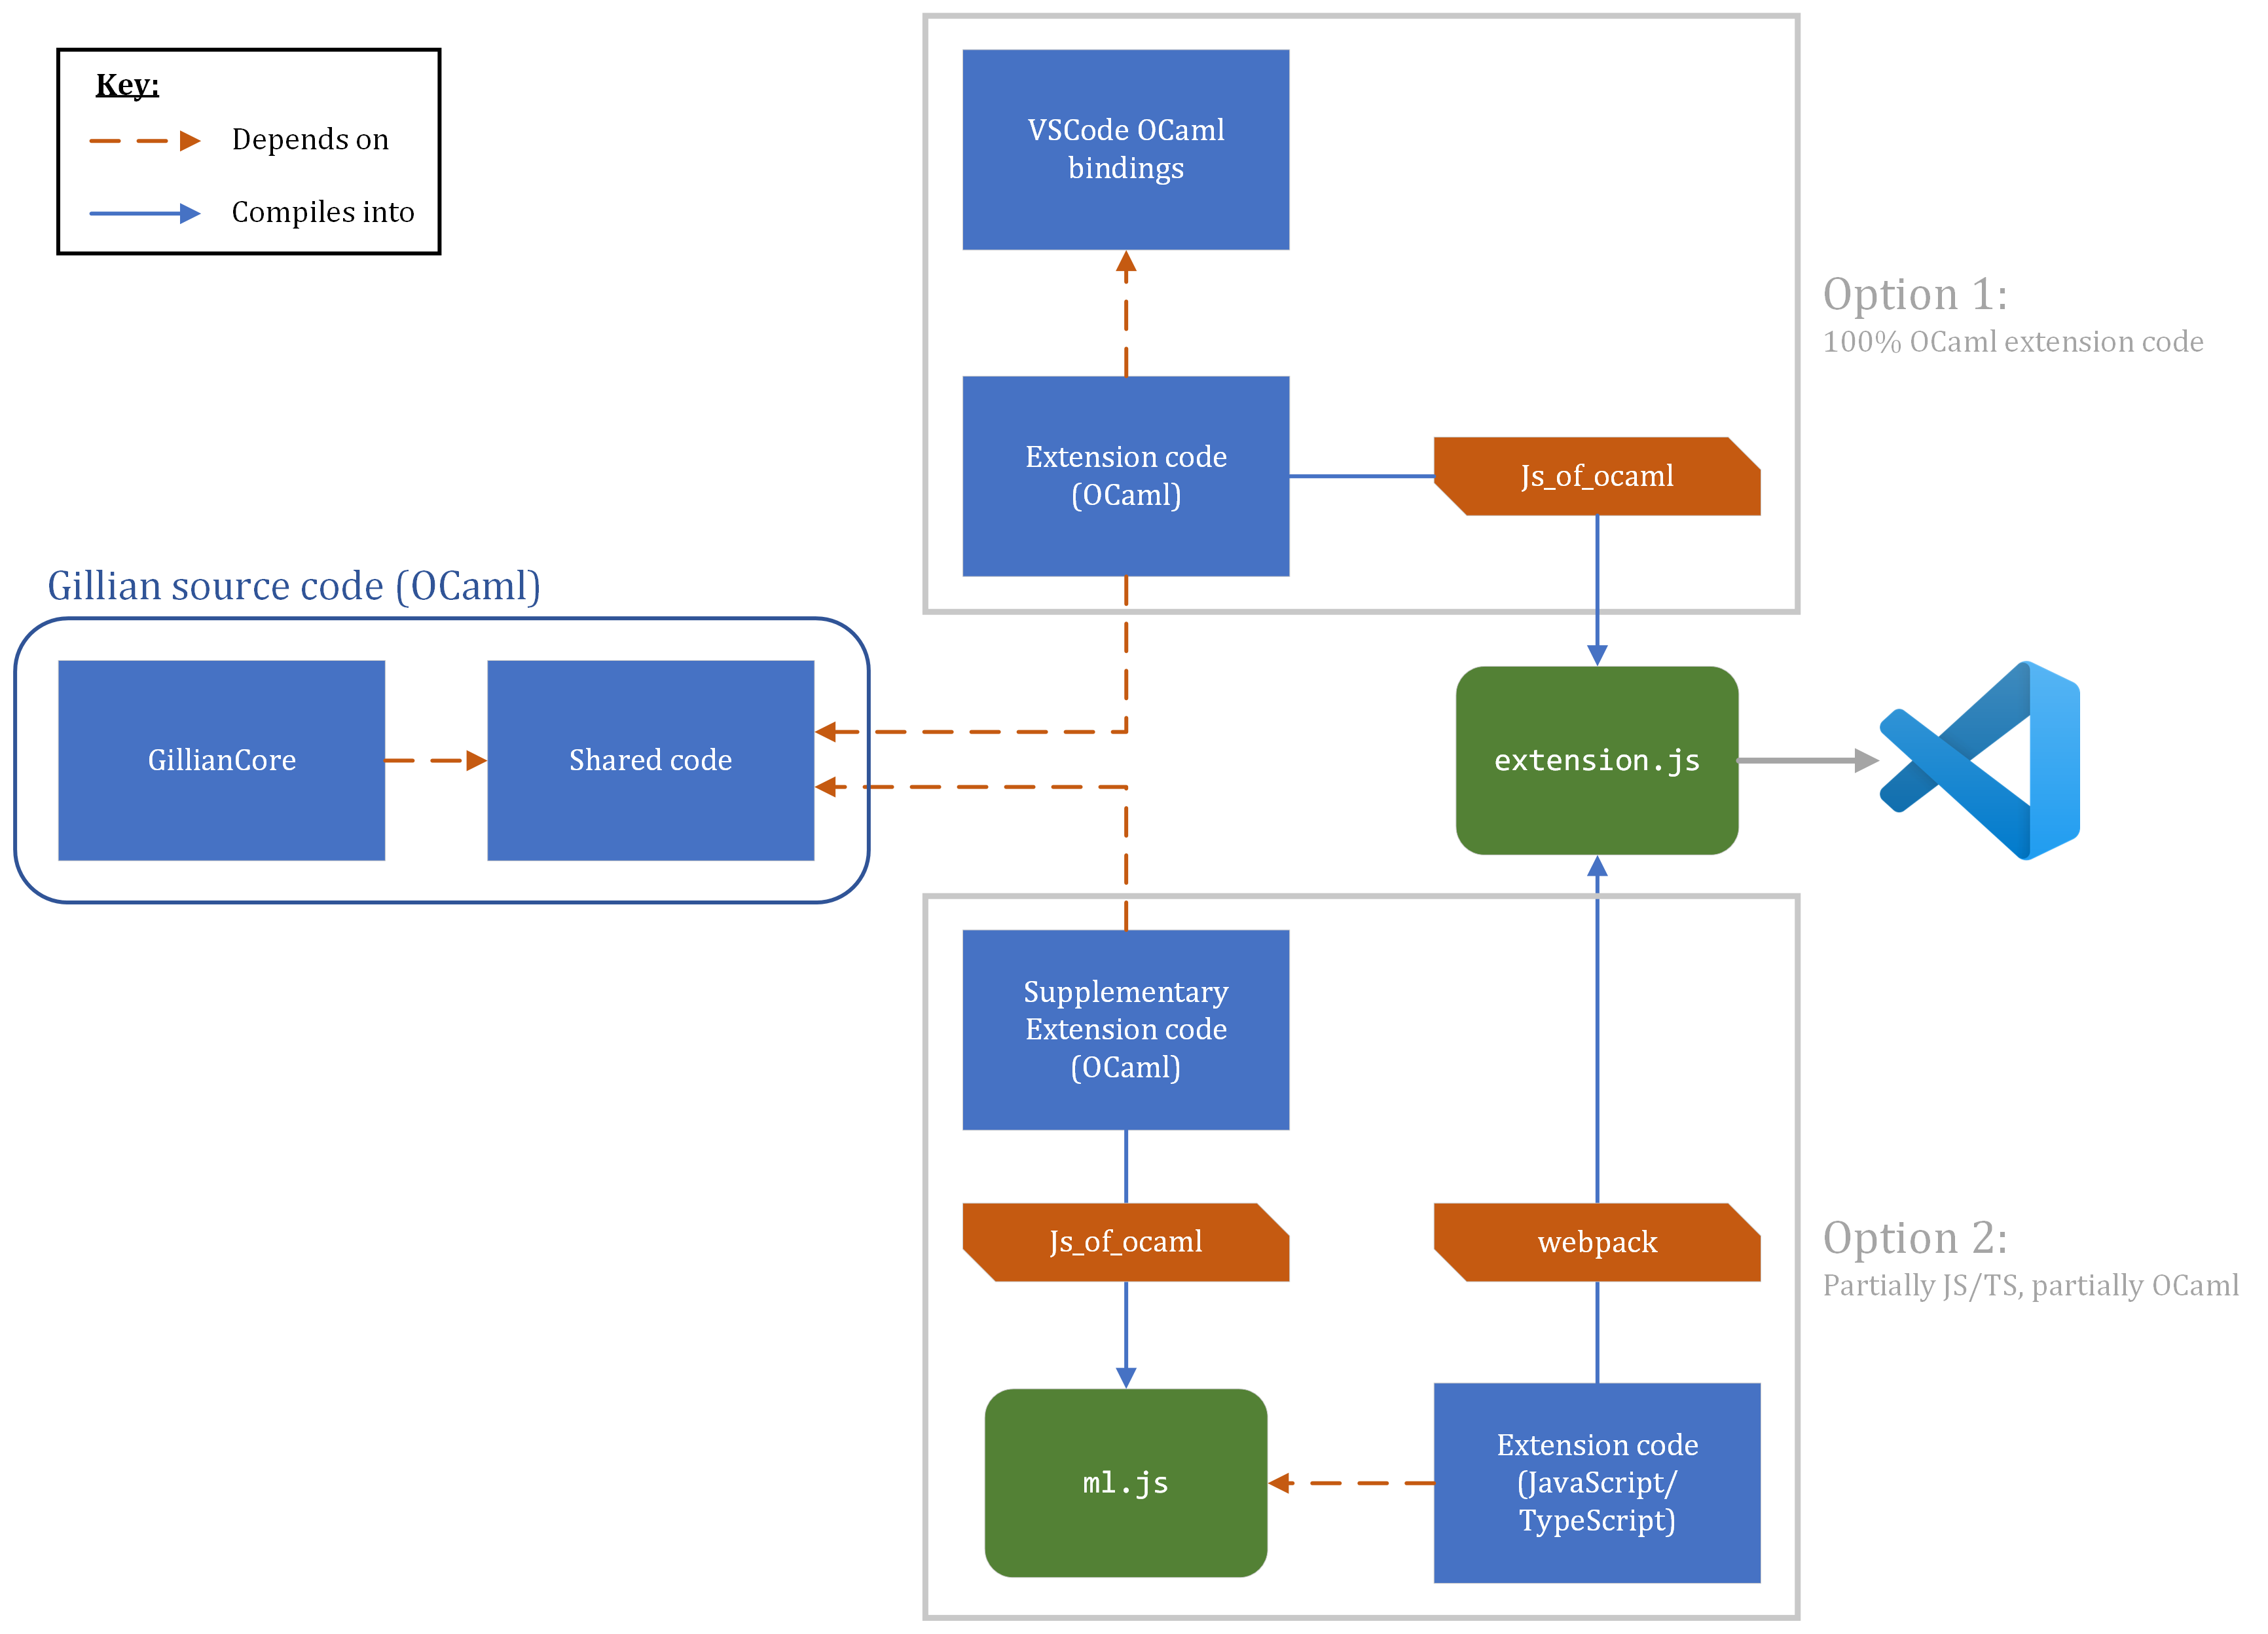
\includegraphics[width=0.8\textwidth]{img/vscode-extension-with-ocaml.png}
  \caption{The process of including OCaml code in a VSCode extension}
  \label{fig:vscode-extension-with-ocaml}
\end{sidewaysfigure}

\myparagraph{Putting it all together}
\label{sec:background:extending-dap}
A combination of DAP custom events and VSCode's Webviews could allow us to move
past DAP's initial limitations. This, however, comes at the cost of creating an
implementation specific to VSCode, eliminating a large benefit of using the DAP
in the first place.

A working example that tests custom DAP commands/events, Webviews and the
inclusion of OCaml code (alongside a Gillian library) is available at
\cite{debugger-experiment}.

\subsection{MagpieBridge}

Similarly to program debugging, adding support for static code analysers to IDEs
is limited by the amount of tools and IDEs that support must be added for. In a
similar notion to the DAP, MagpieBridge~\cite{magpiebridge} is `a framework for
integrating Static Analyses into IDEs and Editors with the Language Server
Protocol'~\cite{magpiebridge-repo}. The \textit{Language Server Protocol}
(LSP)~\cite{lsp} is another of Microsoft's creations, similar to the DAP, which
adds an arbitrary interface bridging IDEs and language tools (syntax checkers,
intellisense, etc.). As an example, MagpieBridge has a provided fully
functional integration for~Infer~\cite{infer-ide}.

A particular feature of MagpieBridge is its ability to serve a configuration
webpage, in which the user can configure the static analysis in their browser
of choice. Unfortunately, this pre-generated page can't contain any custom
content, and can only be used for configuration - this would prohibit advanced
debugging features from being served directly from a MagpieBridge server.

Additionally, the inclusion of MagpieBridge would involve the addition of Java
to the language base of Gillian, increasing complexity of the project and
potentially harming long-term usability.


\begin{figure}
  \centering
  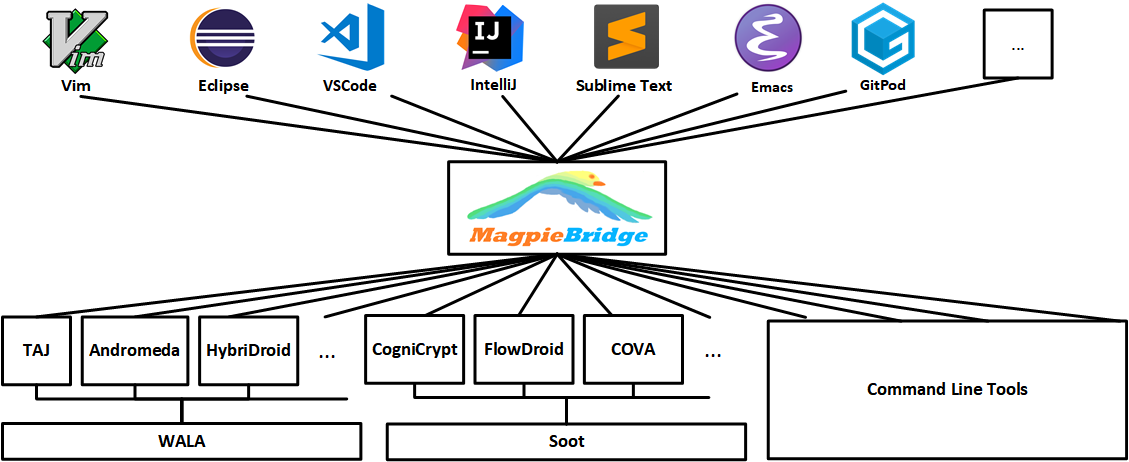
\includegraphics[width=\textwidth]{img/magpiebridge-goal.png}
  \caption{
    The goal of MagpieBridge; bridging static analysis tools with IDEs.
    From~\cite{magpiebridge-repo}.
  }
  \label{fig:magpiebridge-goal}
\end{figure}
